\documentclass{article}
\usepackage{graphicx}
\usepackage[a4paper, hmargin = 2.5cm, vmargin = 2.5cm]{geometry}
\usepackage[english]{babel}

\title{Database project: Travel agency \\ (Milestone 1)}
\author{Oliver Baltisberger, Rachid Flueckiger, Christian Pernet}
\date{\today}

\begin{document}
	\maketitle
	
	\section*{Project description}
	Our project aims to implement a simple customer relationship management database
	for a travel agency. Our ER-Model (see next page) has the following features:
	\begin{itemize}
		\item Each travel agency employee works at a specific branch office (e.g. employee Meier works at the branch office in Zurich) and sells trips to clients.
 		\item A trip can consist of several accommodations (e.g. 2 nights at a hotel in Munich, 3 nights at a hostel in Berlin), transport arrangements (e.g. train from Zurich to Munich, flight from Munich to Berlin) and activities (e.g. football match in Munich, historical city tour in Berlin).
		\item Each trip has one payment (no partial payments allowed), which we consider to be a weak entity (if there is no trip, there is no payment).
	\end{itemize}
	
	\section*{Queries examples}
			
			\begin{enumerate}
				\item List all employees and the number of trips they have sold in the last 12 months.
				\item List all employees working at a particular branch office.
				\item List the sales (i.e. number of trips sold multiplied by their price) generated by an employee. 
				\item Make a list of all clients.
				\item List all clients sorted by the number of trips they have bought.
				\item Make a list of all clients that have booked the same accommodation 	during a defined period.
				\item Make a list of the trips to a specific city/country. 
				\item Make a list of the trips sold during a defined period.
				\item List the average duration/price of a trip.
				\item List the preferred payment method for trips.
				\item List the most popular months for a trip (e.g. more trips are started in July than in November).
				\item Make a list of all accommodations in a country/city. 
				\item Make a list of all accommodation types (e.g. hotel, vacation homes).
				\item What is the most popular accommodation (type) during a defined period?
				\item What type of accommodation/transport/activity are most popular?
			\end{enumerate}	

	\newpage
	
	\section*{ER-Diagram}
	\begin{figure}[htbp]
		\centering
			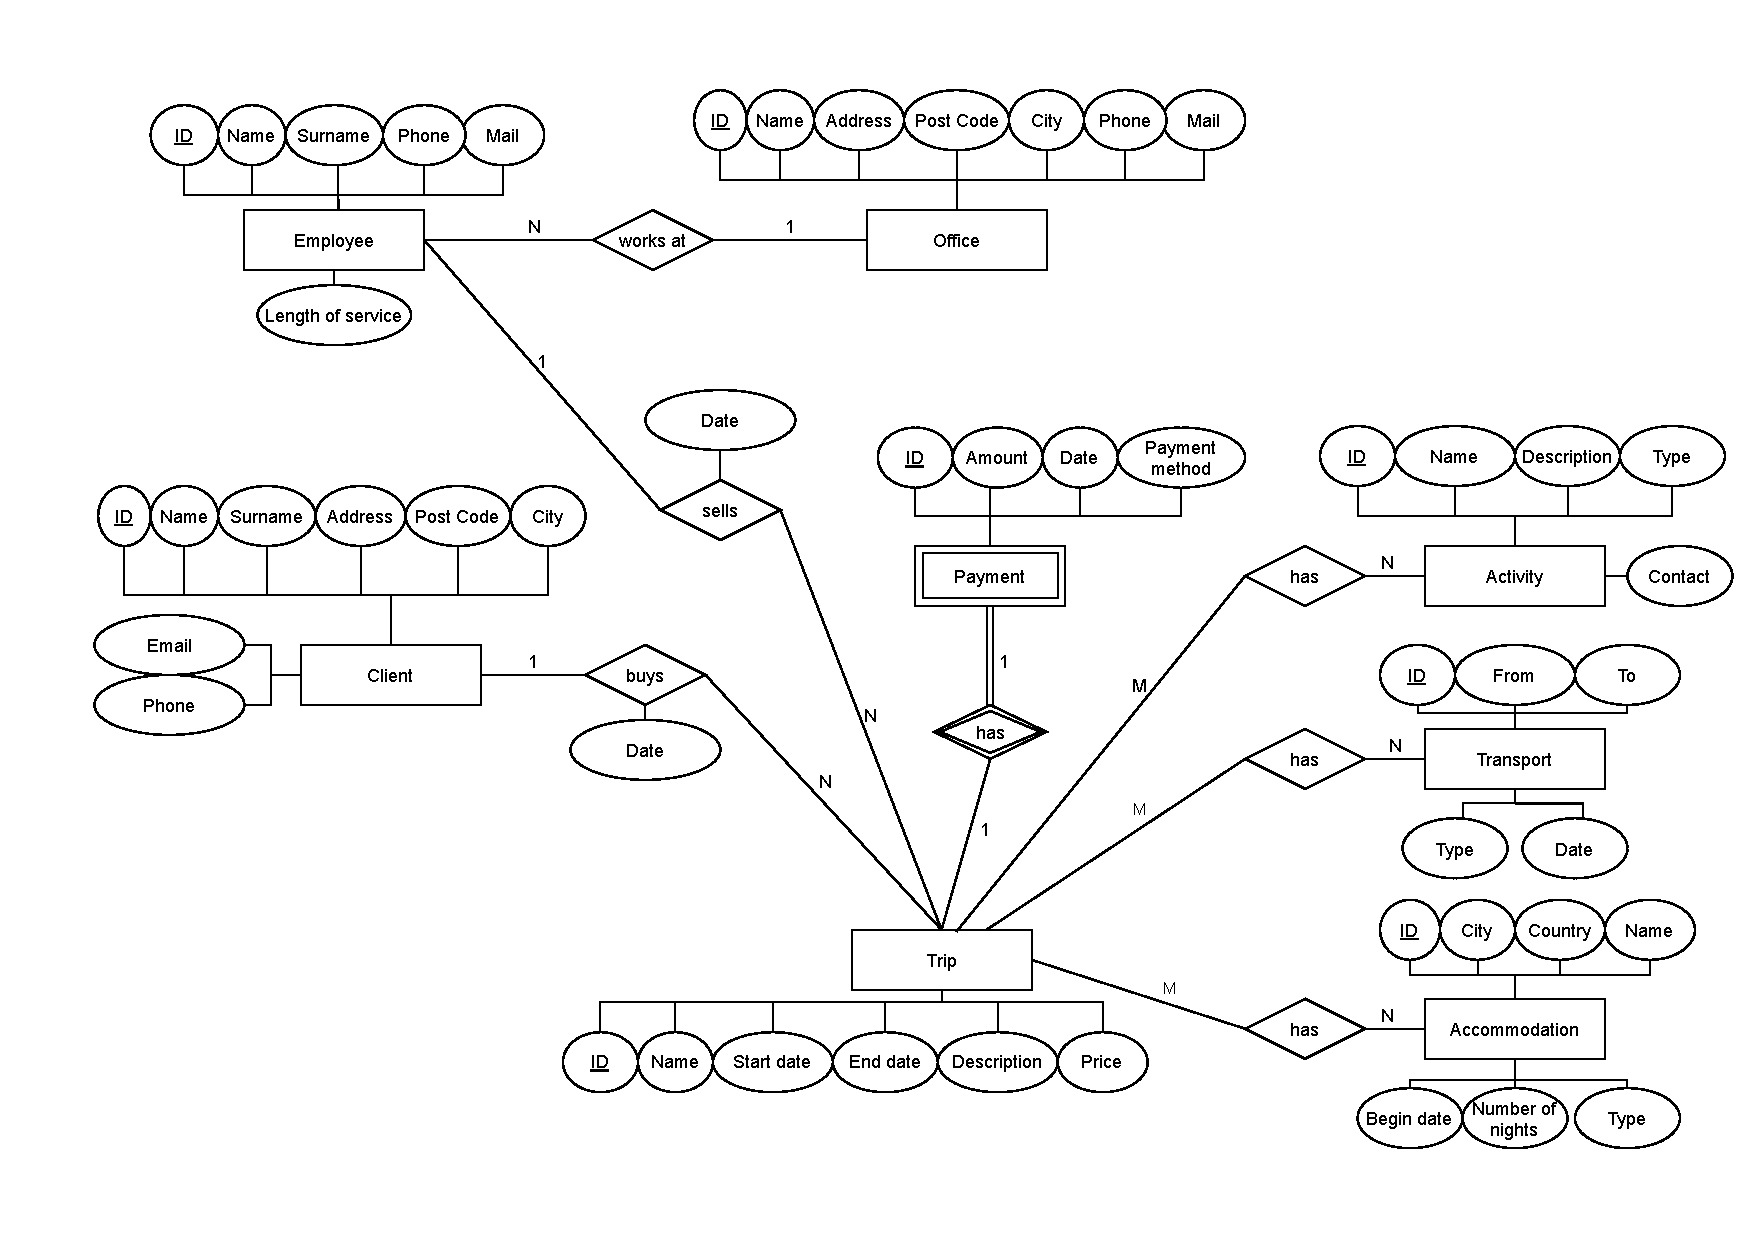
\includegraphics[width=1.15\textwidth, angle=90]{../Proposition 2.pdf}
		\label{ER-Model}
		\caption{Travel agency ER-Model}
	\end{figure}
	

\end{document}